\chapter{Experimental Setup}\label{chap:expSetup}
This section will describe in detail the experimental apparatus used to produce results needed for the analysis carried out in \cref{chap:analyintro}. The complex machinery of the accelerating system is outlined in \cref{sec:method:LHC}. \cref{sec:method:ATLAS} describes the detector system and provides an overview of the filtering and processing of the data acquired by the detector.

\section{The Large Hadron Collider}\label{sec:method:LHC}
The Large Hadron Collider (LHC)~\cite{LHC} operated by the European Organisation for Nuclear Research (CERN) is currently the largest and most powerful particle accelerator in the world. The LHC ring is about \SI{100}{\metre} underground at the French-Swiss border close to Geneva, and has a circumference of \SI{27}{\kilo\metre}. Predominantly performing proton-proton (\protonproton) collisions with a design centre-of-mass collision energy of $\sqrt{s} = \SI{14}{\tera\electronvolt}$ and an instantaneous luminosity of \SI{e34}{\centi\metre^{-2} \second^{-1}}. Whilst the LHC also allows to accelerate heavy ions (e.g.\ Pb and Xe), the heavy-ion program is not discussed further, as only \protonproton collision data is used for the presented studies in this thesis. 

The LHC is supported by a chain of pre-accelerators which are used to ramp protons to the required input energy of \SI{450}{\giga\eV}~\cite{LHCInjectorChain,LHCFacts}. A schematic of the LHC accelerator chain is shown in \cref{fig:method:CERN-complex}. The process begins by stripping off orbiting electrons from hydrogen to obtain protons. This is done by the \emph{Linac 2}, a linear accelerator which also accelerates the protons to an energy of \SI{50}{\mega\eV}. These proton beams are then fed into the \emph{Proton Synchrotron Booster} (PSB), first of a series of circular accelerators that accelerate the protons to an energy of \SI{1.4}{\giga\eV}. The beams then enter the \SI{628}{\meter} long \emph{Proton Synchrotron} (PS) where the proton beams are accelerated to a beam energy of \SI{25}{\giga\eV} and injected into the \emph{Super Proton Synchrotron} (SPS). At the penultimate stage of the acceleration in the \SI{6.9}{\kilo\meter} ring of the SPS, the proton beam reaches the required beam energy of \SI{450}{\giga\eV} arranged in 240 bunches. After the SPS, the protons injected into counter-circulating LHC rings to be accelerated to their maximum energy, where collisions under stable conditions are achieved.
\begin{figure}
    \centering
    \includegraphics[width=\textwidth]{images/CCC-v2018-print-v2.pdf}
    \caption[The CERN accelerator complex]{The CERN accelerator complex in 2018, including the LHC and the pre-accelerators~\cite{CERNComplex}.}
    \label{fig:method:CERN-complex}
\end{figure}

There are a total of 1232 dipole magnets installed in the LHC that are used to steer the proton beams around each ring. For proton energies of \SI{7}{\tera\eV}, a magnetic field of \SI{8.3}{\tesla} is required in these dipoles. To keep the beams focused and achieve small beam size at the 
interaction point quadrupole and higher-order magnets are used. 

In total there are a maximum of 3564 possible bunch positions with a spacing of \SI{25}{\nano\second} available at the LHC. However, due to rise-time constraints of the injector and beam-dump kicker magnets, this is reduced to 2808 with approximately $10^{11}$ protons per bunch. The filling choice of the LHC ring is the so-called bunch scheme. The bunches are typically clustered in what are called bunch trains.

The two circulating protons beams intersect at four interaction points where the main experiments are installed around the LHC. CMS~\cite{CMS} and ATLAS~\cite{ATLAS}, two general-purpose detectors allow precision measurements of SM processes, including the properties of the Higgs boson, and allow for the search for physics beyond the SM. LHCb~\cite{LHCb} and ALICE~\cite{ALICE} are two lower rate specialised detectors studying the properties of flavour physics and heavy-ion physics, respectively. To study the properties of particles with very low scattering angles from the beam (i.e. forward physics), TOTEM~\cite{totem:2008zza} and LHCf~\cite{LHCf:2008zz}, two additional smaller experiments were also installed at the LHC.

\section{The ATLAS detector}\label{sec:method:ATLAS}

The ATLAS experiment is the world's largest general-purpose detector. Situated at one of the interaction points around the LHC, it is \SI{4}{\meter} in length and \SI{25}{\meter} in height and weighs approximately \SI{7000}{\tonne}. ATLAS consists of several sub-detector systems arranged in sequential layers. Several electromagnet systems provide a strong magnetic field coverage across the detector body. The \emph{Inner Detector (ID)} located nearest to the interaction point, provides position and momentum information for charged particles emerging from the collisions. Two calorimeter systems, the \emph{Electromagnetic Calorimeter} and the \emph{Hadronic Calorimeter} are used to measure the energy of charged and neutral particles. The \emph{Muon Spectrometer} forming the outermost layer of the detector, provides momentum measurements for muons. An overview of the ATLAS detector and its subsystems is outlined in \cref{fig:method:ATLAS}.

\begin{figure}
    \centering
    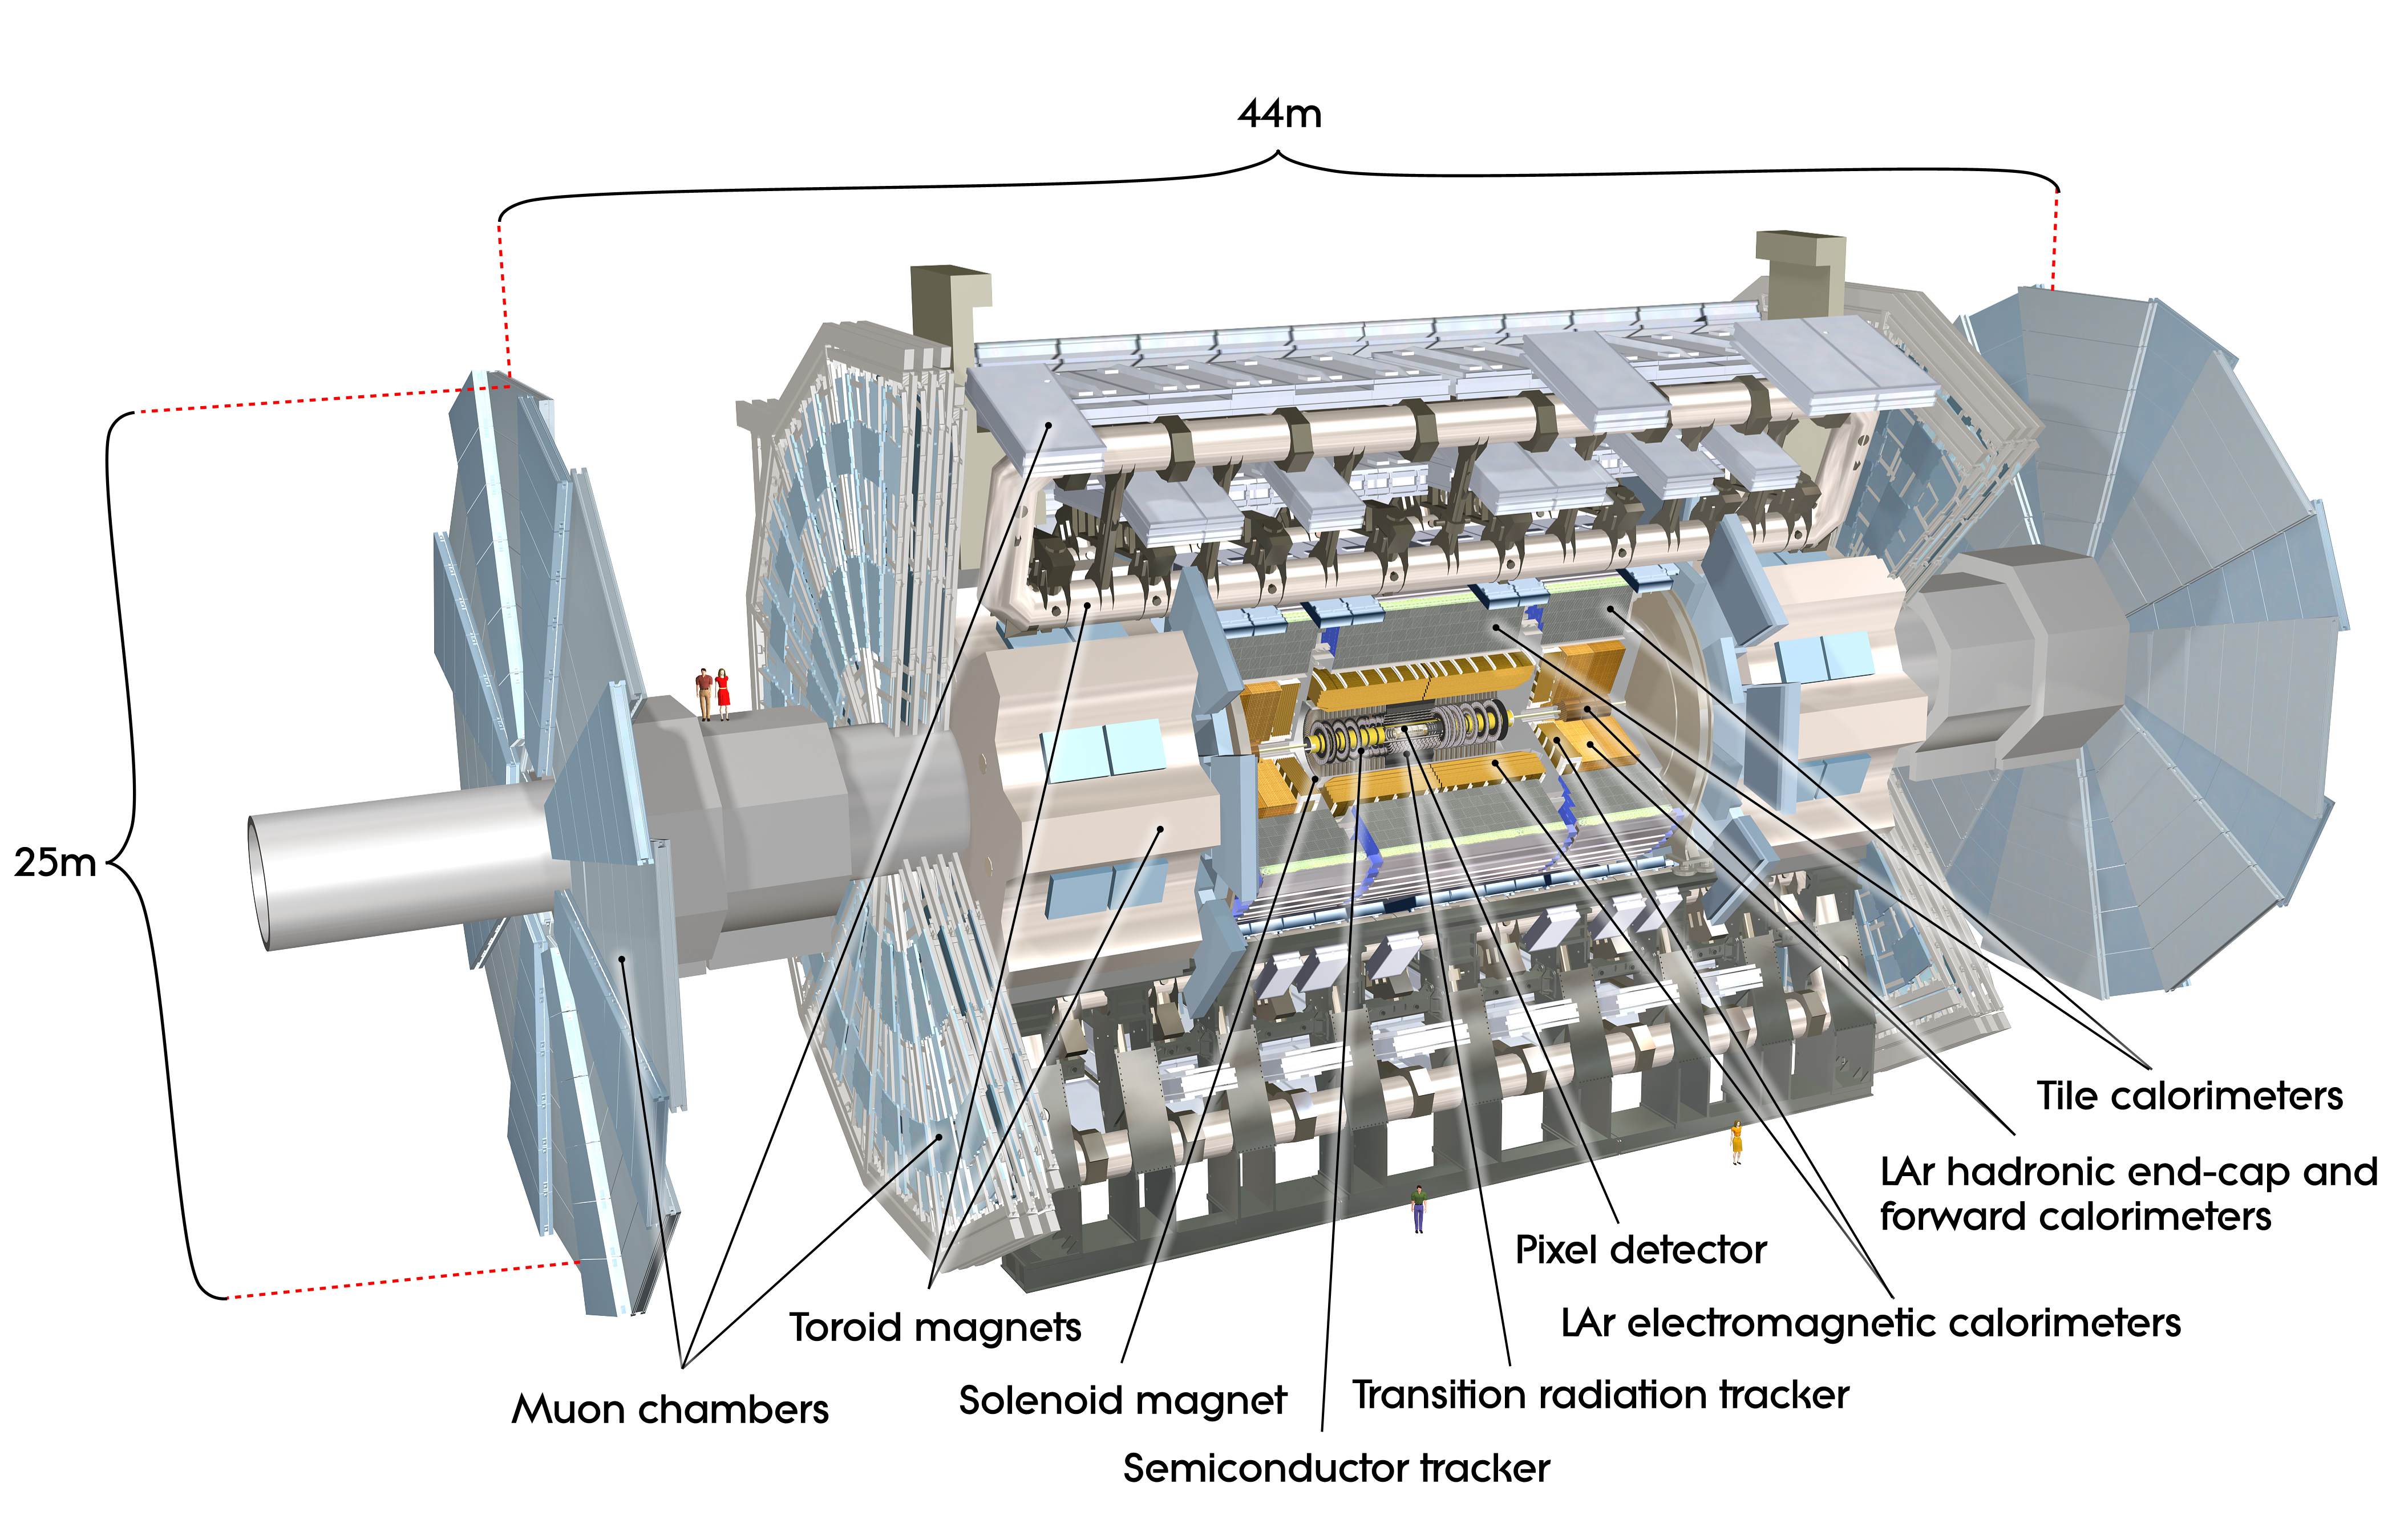
\includegraphics[width=\textwidth]{images/ATLAS.png};
    \caption[Schematic of the ATLAS detector]{Schematic overview of the ATLAS detector highlighting the major subdetector components within it~\cite{ATLASImage}.}
    \label{fig:method:ATLAS}
\end{figure}

\subsubsection{ATLAS coordinate system and kinematic quantities}

ATLAS uses a right-handed coordinate system with its origin in the centre of the detector at the interaction point. The x-axis is aligned such that it points towards the centre of the LHC ring, the positive y-axis points upwards, and the z-axis is defined going along the beam-pipe. An angular system is used where \emph{r} is the radial distance from the point of interest, \emph{$\phi$} is the azimuthal angle in the x-y transverse plane and the polar angle \emph{$\theta$}. \emph{Pseudorapidity}, $\eta = -\log\tan\frac{\theta}{2}$, is used as a dimensionless measure of \emph{$\theta$}. The change in \emph{$\eta$} is invariant under Lorentz boosts along the beam axis. The distances between objects are defined in the azimuthal-pseudorapidity  space as $\Delta R^2 = \Delta \eta^2 + \Delta \phi^2$. 

The momentum of an object is expressed in Cartesian coordinates as $\textbf{p} = (p_x,p_y,p_z)$, where $p_x$, $p_y$ and $p_z$ are the momentum in the x,y and z directions, respectively. The missing transverse momentum of an object, \pt, is defined as the projection of momentum in the x-y plane. transverse momentum is given by
\begin{equation}
    \pt = \sqrt{ p_{x}^{2} + p_{y}^{2}}~.
\end{equation}

\subsection{Inner Detector}\label{sec:method:ID}
The Inner Detector (ID)~\cite{ATLAS:ID-TDR}, embedded in a \SI{2}{\tesla} solenoid magnetic field, allows for the tracking of charged particles near to the interaction point. It is designed to achieve high-precision measurements of momentum and measurements of primary and secondary vertices of collisions in the range $\abs{\eta} \leq 2.5$. It is composed of three independent detector technologies: the \emph{pixel detector}, \emph{semi-conductor tracker (SCT)}, \emph{transition radiation tracker (TRT)} and the \emph{insertable B-layer} as shown in ~\cref{fig:method:ATLAS:ID}. 
\begin{figure}[!htpb]
    \centering
    \begin{subfigure}[b]{0.49\textwidth}
        \centering
        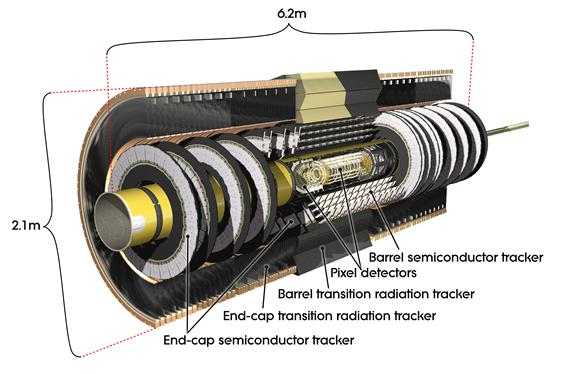
\includegraphics[width=\textwidth]{images/ATLAS_ID_no_IBL}
        \label{fig:ID1}
    \end{subfigure}
    \begin{subfigure}[b]{0.49\textwidth}
        \centering
        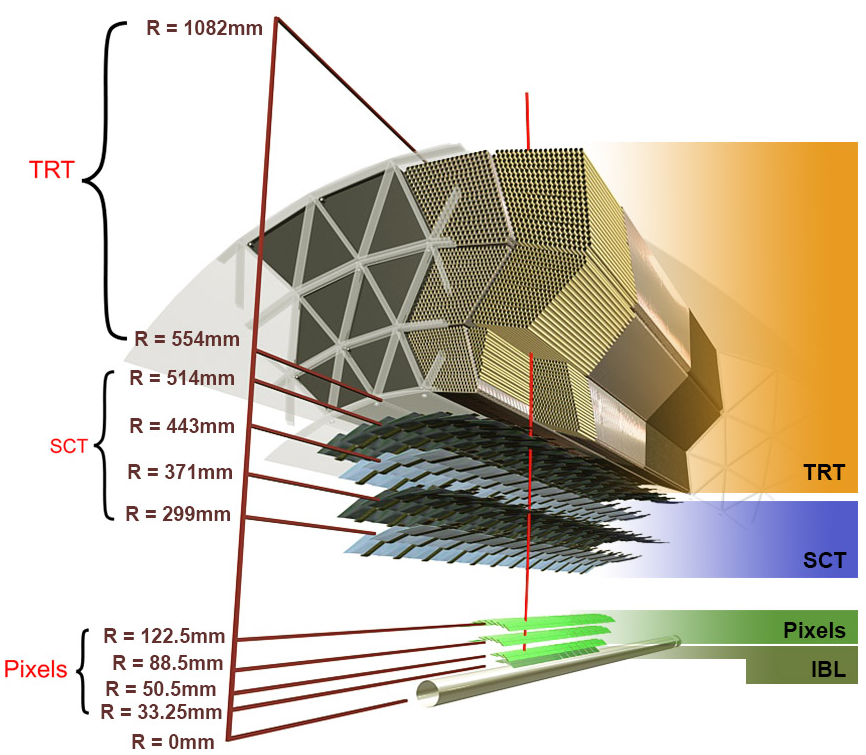
\includegraphics[width=\textwidth]{images/ID_withIBL}
        \label{fig:ID2}
    \end{subfigure}
    \caption[Illustration of the ATLAS inner detector]{Illustration of the ATLAS inner detector, containing the pixel detector, semiconductor tracker (SCT), transition radiation tracker (TRT)and the \emph{insertable B-layer}. The components of the inner detector are shown along the beam-pipe (left) and a slice of the inner detector (right).}
    \label{fig:method:ATLAS:ID}
\end{figure}
% \begin{figure}
%     \centering
%     \begin{tikzpicture}
%         \node [anchor=south west,inner sep=0] (image) at (0,0) {\includegraphics[width=\largefigwidth]{images/inner_detector}};
%         \node [anchor=west] (endcap_sct) at (10,3.5) {\small End-cap SCT};
%         \draw (endcap_sct) to (10.1,5.9);
%         \node [anchor=west] (barrel_sct) at (8.5,2.9) {\small Barrel SCT};
%         \draw (barrel_sct) to (8,4.5);
%         \node [anchor=west] (pixel) at (7,2.2) {\small Pixel detector};
%         \draw (pixel) to (7,4.9);
%         \node [anchor=west] (barrel_trt) at (5.5,1.5) {\small Barrel TRT};
%         \draw (barrel_trt) to (6.5,3);
%         \node [anchor=west] (endcap_trt) at (3.5,0.8) {\small End-cap TRT};
%         \draw (endcap_trt) to (4.6,2.2);
%     \end{tikzpicture}
%     \caption[Illustration of the ATLAS inner detector]{Illustration of the ATLAS inner detector, containing the pixel detector, semiconductor tracker (SCT), and transition radiation tracker (TRT). The \emph{insertable B-layer}, installed in 2014, is not shown~\cite{ATLASIDImage}.}
%     \label{fig:method:ATLAS:ID}
% \end{figure}

\subsubsection{Pixel detector}
The innermost part of the ID closest to the interaction point is the pixel detector. It provides high-resolution information on the location of charged particles. It is formed of four concentric cylindrical layers, the \emph{Insertable B-Layer (IBL)}~\cite{ATLAS:IBL-TDR}, added in 2014, and three additional layers in the barrel region. The layers of the pixel detector are based on silicon semiconductor technologies. This allows the detection of charged particles when traversing through the doped silicon, where an electron-hole pair is formed resulting in a current. The semiconductor sensors are arranged in a grid and provide fine granularity position information. The IBL pixels are situated at a distance of $R = \SI{33.25}{\milli\meter}$ from the centre of the beam pipe and have a size of $\SI{50}{\micro\meter} \times \SI{250}{\nano\meter}$ in $R \times \phi, z$, with an intrinsic resolution of $\SI{8}{\micro\meter} \times \SI{40}{\micro\meter}$. The outer layer pixels measure $\SI{50}{\micro\meter} \times \SI{400}{\nano\meter}$ with an intrinsic resolution of $\SI{10}{\micro\meter} \times \SI{115}{\micro\meter}$~\cite{ATLAS:ID-TDR}. With the addition of the IBL, the position resolution of primary and secondary vertices was improved to \SI{10}{\nano\meter} in R$\phi$ and \SI{115}{\micro\meter} in z~\cite{Rosa}. 

\subsubsection{Semiconductor tracker}
Based on silicon sensors, the SCT is located \SI{299}{\nano\meter} from the interaction point. The SCT detects charged particles through the same mechanism as the pixel detector. However, instead of pixels, it uses long strip sensors arranged in four cylindrical layers in the barrel region and nine disks in the end-caps. The SCT strip modules are arranged in pairs with a \SI{40}{\milli\radian} relative angle, where each module consists of several SCT strips. Therefore, it provides two independent hits that allows for the measurement of $(r,\phi)$. In the barrel region for each track four space points with an intrinsic resolution of \SI{17}{\micro\meter}, in R$\phi$ and \SI{580}{\micro\meter} in z can be obtained.

\subsubsection{Transition radiation tracker}
Located \SI{563}{\milli\meter} from the interaction point the TRT is the outermost component of the ID. The TRT is formed of approximately 370000 gas-filled straw tube detectors. Each straw tube is a hollow cylinder with a diameter of \SI{4}{\milli\meter} containing a central tungsten wire filled with a gas mixture predominantly made out of Xenon. The tungsten wire along with the tube forms a capacitor, where the wire is the anode, and the surrounding tube acts as the cathode. When charged particles pass through the tube, the gas is ionised, producing an avalanche of electrons. The avalanche of electrons is detected as an electric current in the wire. The TRT has 73 straw planes in the barrel region, spaced horizontally at a distance $\SI{563}{\milli\meter} < R < \SI{1066}{\milli\meter}$ and $\abs{z} < \SI{712}{\milli\meter}$ from the interaction point, and 160 straw planes in the end-caps orientated in the radial direction. This results in on average 30 to 40 hits detected per particle by the TRT. The TRT straws have an intrinsic resolution of \SI{130}{\micro\meter} in the $R\phi$ plane. 

The TRT additionally consists of polypropylene fibres and polypropylene foils interleaved between the straw tubes in the barrel and end-cap modules respectively. Charged particles passing through the polypropylene undergo transition radiation. Transition radiation is produced when ultra-relativistic particles travel through the boundary of two materials with different dielectric constants. This radiation corresponds to photons and is proportional to the relativistic factor, $\gamma$, of the incident particle. Therefore, it will be higher for electrons compared to pions. This difference is crucial for differentiating between electrons and pions. 

% \subsubsection{Performance}

% Precise tracking information is needed to measure the properties of particles expected in final states of analyses. Using the information from the ID with the exclusion of the IBL, the expected resolution is given by [REF]
% \begin{equation}
%    \sigma(\frac{1}{p_{T}}) \cdot p_{T} = 0.036 \% \cdot p_{T}[GeV] \oplus 1.3 \%
% \end{equation}

\subsection{Calorimeters}\label{sec:method:Cals}
The ATLAS calorimetry system consists of the electromagnetic and the hadronic calorimeters and is located closest to the beam pipe after the ID outside of the solenoid magnet. They are designed to measure the position and energy of particles emerging from the interaction point. They use materials which have a high probability of particles interacting with them. The electromagnetic and hadronic calorimeters are specialised in measuring the energies of $\gamma$ and $e$, and hadrons, respectively. Neutral particles like $\gamma$ and neutral hadrons, which do not induce a signal in the ID, can be identified in the calorimeters. This allows for nearly all Standard Model particles to be identified except for weakly interaction neutrinos and $\mu$, which have minimal interactions within the distance of the calorimeters and the interaction point. 

High energy particles produce particle showers of lower-energy particles that travel through the calorimeter material. Therefore, it is essential to ensure that particle showers are contained within the calorimeters when designing them. The depth of a calorimeter material can be characterised by a particles radiation length ($\chi_{0}$), and its nuclear interaction length ($\lambda$). Nuclear interaction length is defined as the mean distance a particle travels in a medium before undergoing a nuclear interaction. Due to electromagnetic interactions with the surrounding material, over one radiation length, a particle loses on average $e^{-1}$ its original energy. 

ATLAS using sampling calorimeters for both the electromagnetic and hadronic calorimeters. The Calorimeter materials have been selected to either be ionised or scintillate when particle a particle shower enters, which results in a measurable electrical signals. A particles energy can be calculated by summing the total radiation produced by a shower in the active layers. 

\subsubsection{Electromagnetic calorimeter}
The electromagnetic calorimeter is designed to fully measure the energies of electrons (and positrons), and photons. Measurements of the energies of particles are made by inducing electromagnetic showers when the particle interacts with a dense material. For electrons, the shower is primarily initiated by bremsstrahlung, while for photons it is initiated by pair production. Shower particles are then detected by the detecting layers of the calorimeter interleaved with layers of dense material.

\begin{figure}
    \centering
    \begin{tikzpicture}
        \node[anchor=south west,inner sep=0] (image) at (0,0) {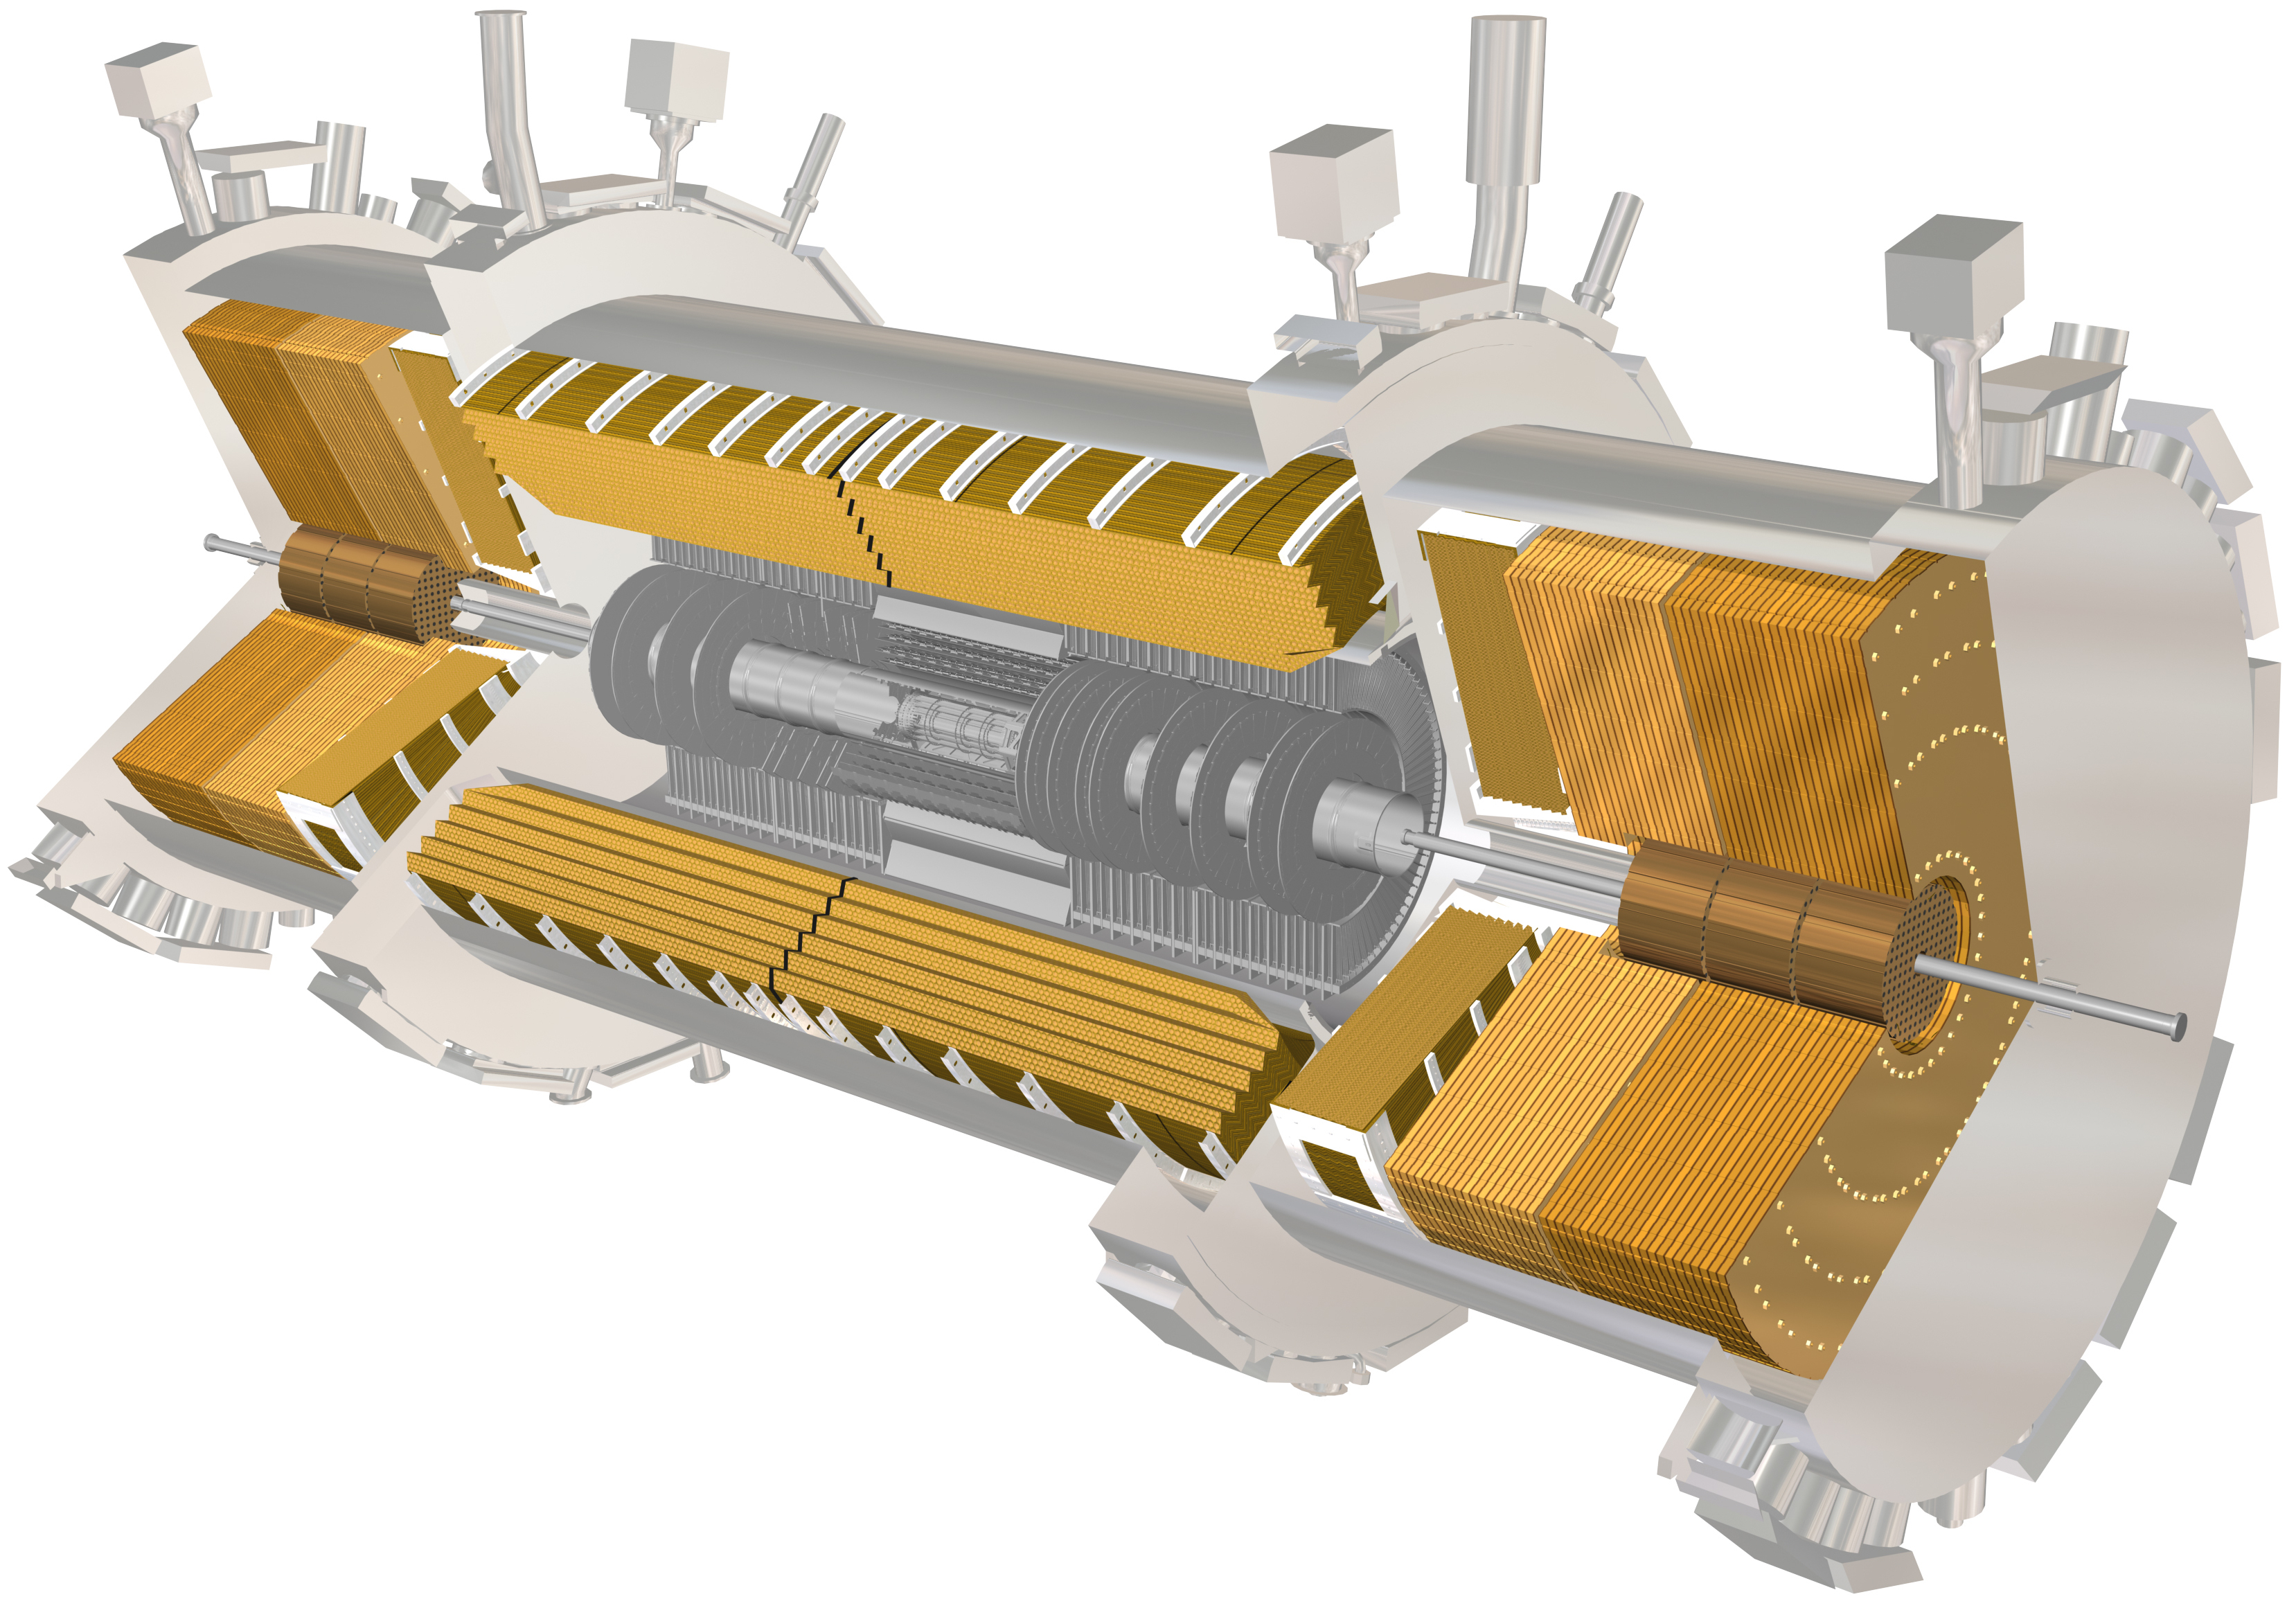
\includegraphics[width=\largefigwidth]{images/lar.jpg}};
        \node[anchor=west,align=center] (hec) at (-2.0,2.3) {\small Hadronic end-cap\\ calorimeter};
        \draw (hec) to ++(2,2.5);
        \node[anchor=west,align=center] (fcal) at (8.5,-0.8) {\small Forward calorimeter};
        \draw (fcal) to ++(-1.4,4.4);
        \node[anchor=west,align=center] (ecal) at (0,1) {\small Barrel electromagnetic\\ calorimeter};
        \draw (ecal) to ++(1.3,2.6);
        \node[anchor=west,align=center] (emec) at (4,0) {\small Electromagnetic end-cap\\ calorimeter};
        \draw (emec) to ++(1.1,3);
        \clip (current bounding box.south west) rectangle ($(current bounding box.north east)+(1.5,0)$);
    \end{tikzpicture}
    \caption[Illustration highlighting the liquid argon components of the ATLAS calorimeters]{Illustration highlighting the liquid argon components of the ATLAS calorimeters~\cite{ATLASLarImage}.}
    \label{fig:method:ATLAS:LAr}
\end{figure}

The electromagnetic calorimeter uses liquid argon (LAr) as its scintillator material and lead plates as its shower inducing material. Liquid argon component of the calorimeter was chosen due to its stability of response over a long period while being exposed to radiation~\cite{ATLAS:LAr-TDR}. It is divided into the barrel and end-cap regions highlighted in \cref{fig:method:ATLAS:LAr}. 

In the barrel region, the electromagnetic calorimeter is split into three regions of different granularity. The innermost layer of the calorimeter has a fine granularity in $\eta$. The thickest layer of the electromagnetic calorimeter is the second layer, arranged in a square grid, which aids in locating the primary vertices of particles. Combining the measurements of the first two layers allows for locating the origin of neutral particles that do not leave tracks in the ID. The final layer, with the largest granularity, is used to estimate the energy lost beyond the electromagnetic calorimeter and to distinguish between electromagnetic and hadronic showers. A sketch of the barrel module is shown in \cref{fig:method:ATLAS:ECal}, where the cell granularity of each section is visible.
\begin{figure}
    \centering
    \begin{tikzpicture}
        \node[anchor=south west,inner sep=0] (image) at (0,0) {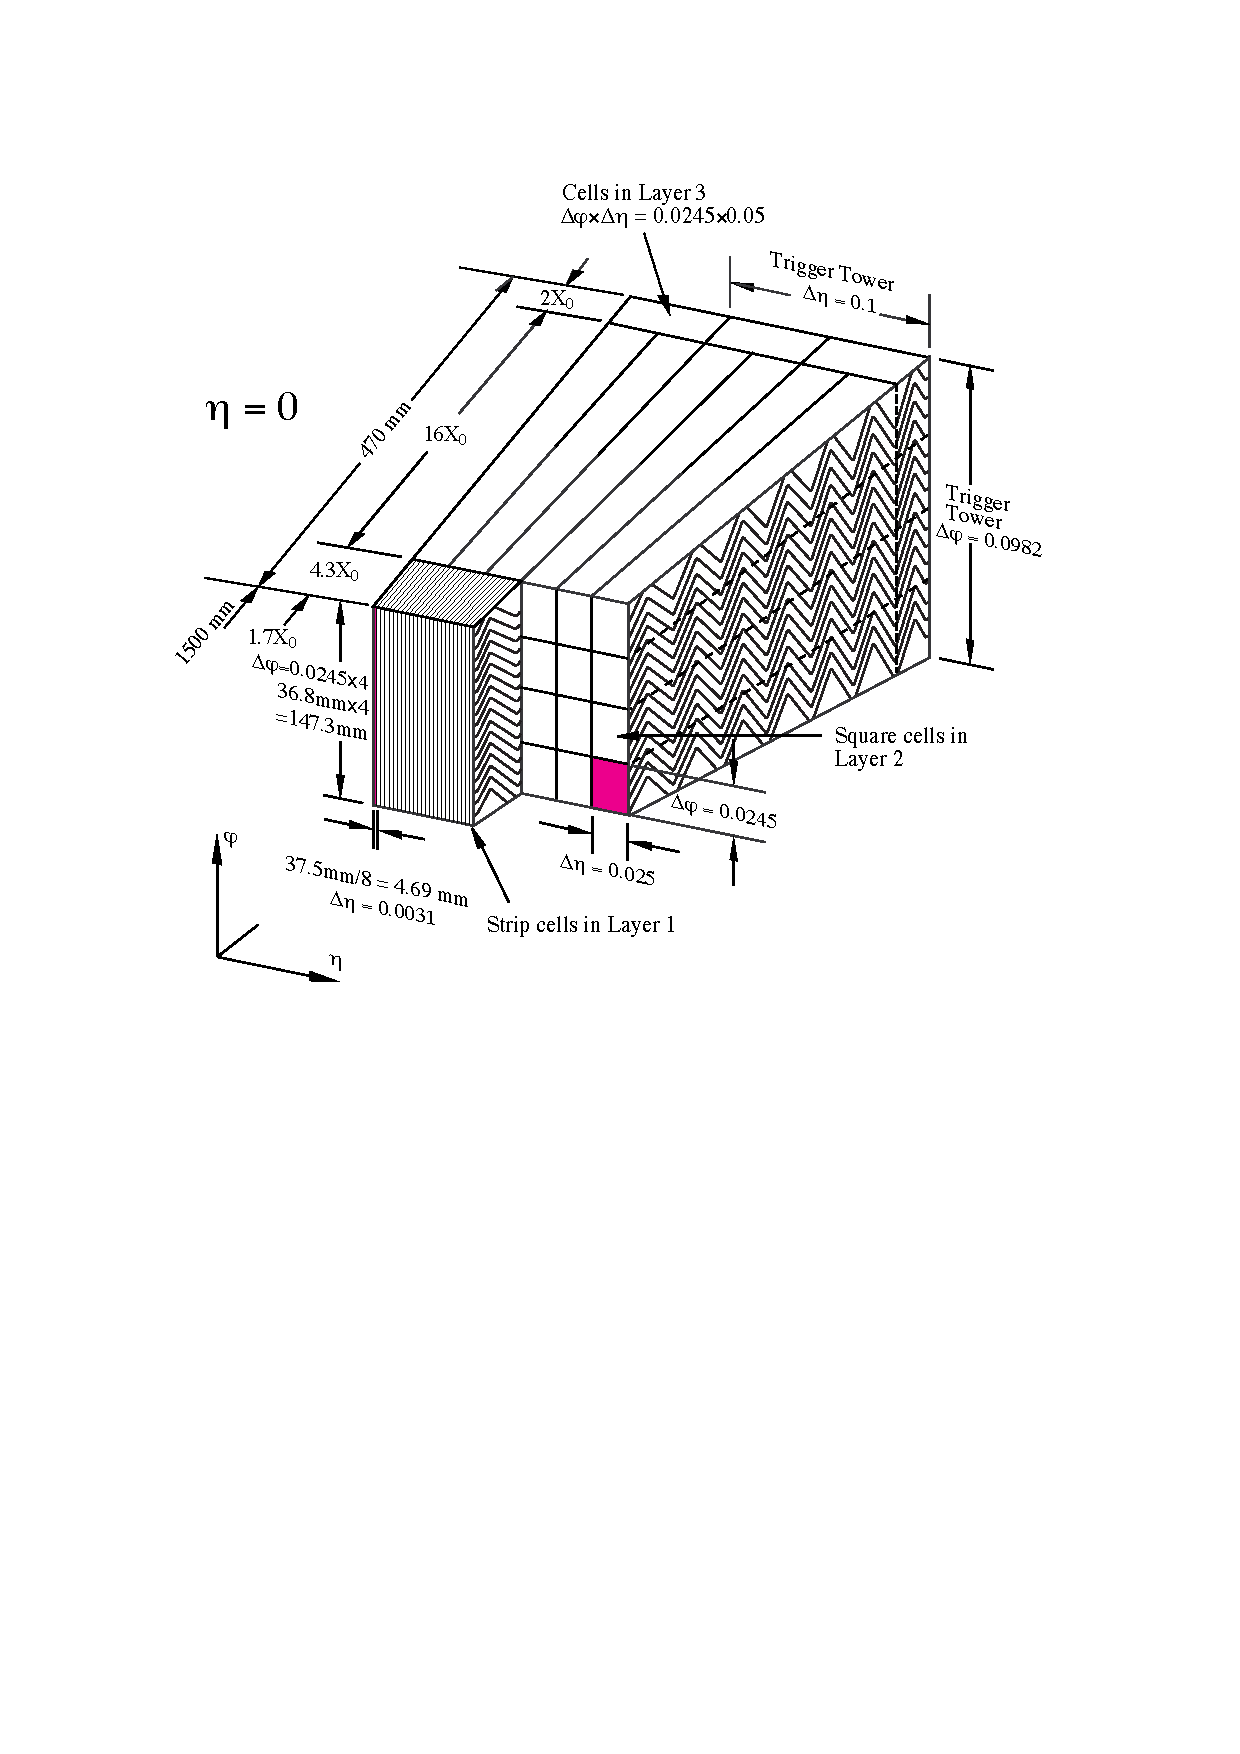
\includegraphics[scale=0.9]{images/calo.pdf}};
    \end{tikzpicture}
    \caption[Drawing showing a section of the barrel electromagnetic calorimeter]{Drawing showing a section of the barrel electromagnetic calorimeter.
    The liquid argon cells are arranged into three distinct layers, with granularity decreasing for larger radius~\cite{ATLAS}.}
    \label{fig:method:ATLAS:ECal}
\end{figure}

In the forward region, each end-cap electromagnetic calorimeter consists of two coaxial wheels separated by \SI{3}{mm}. The inner wheels are constructed similarly to the barrel calorimeters shown in \cref{fig:method:ATLAS:ECal}. The other wheels do not have a third layer, and the majority of the thickness is composed of the first two layers. 

\subsubsection{Hadronic calorimeter}
The hadronic calorimeter, like the electromagnetic one, is a sampling calorimeter. Unlike the electromagnetic calorimeter, it uses steel as the shower-inducing material and scintillating plastic tiles~\cite{ATLAS:tile-TDR}. The hadronic showers originate from interactions of incoming hadrons with the shower inducing material. The tile calorimeter sits in the barrel region at $\abs{\eta} < 1.7$ where it is divided into the tile barrel $\abs{\eta} < 1.0$ followed by the extended barrels covering $ 0.8 < \abs{\eta} < 1.7 $. The barrel and extended barrels are divided azimuthally into 64 modules. On the edges of the tiles, wavelength shifting fibres are used to extract signals by guiding them into photomultiplier tubes. 

The hadronic end-cap calorimeter covers $1.5 < \abs{\eta} < 3.2$ using LAr technology. It consists of two wheels per end-cap and uses copper as the shower-inducing material. In each end-cap two independent wheels are placed with \SI{50}{\milli\meter} copper plates. A greater containment is achieved compared to the tile calorimeter by placing 12 nuclear interaction lengths of material before the muon spectrometers. 

\subsubsection{Forward calorimeters}
The forward calorimeter provides additional coverage in the range $3.1 < \abs{\eta} < 4.9$ and is designed to measure the energies of both electromagnetic and hadronic showers~\cite{ATLAS:LAr-TDR}. It consists of three modules, each using LAr as the detecting material. Copper rods are placed parallel to the beam axis in the innermost layer, is optimised for electromagnetic showers. Tungsten rods are used for the second and third layers as the shower-inducing material to measure the energy of hadronic particles. 

\subsubsection{Performace}
Many analyses in ATLAS require an excellent energy resolution. Based on test beam-data, the calorimeter energy resolution is summarized in ~\cref{tab:method:ATLAS:ecalperf}.

\begin{table}
    \begin{tabular}{c|c|c}
         & Detector component & Resolution \\
        \midrule
       EM & Barrel and end-cap &  $\sigma_E/E = 10\%/\sqrt{E} \oplus 0.7\%$\\
        
       Hadronic & Barrel and end-cap & $\sigma_E/E = 50\%/\sqrt{E} \oplus 3\%$ \\
                & Forward &  $\sigma_E/E = 100\%/\sqrt{E} \oplus 10\%$\\
    \end{tabular}
    \caption[ATLAS calorimetry energy resolution]{ATLAS calorimetry energy resolution, as obtained from beam-test data~\cite{ATLAS:testbeam-calo,ATLAS:testbeam-hcal}.}
    \label{tab:method:ATLAS:ecalperf}
\end{table}

\subsection{Muon spectrometer}\label{sec:method:MS}

The outermost portion of the ATLAS detector consists of the muon spectrometer~\cite{ATLAS:muon-TDR} as shown in \cref{fig:method:ATLAS:muons}. Muons can traverse through most of the ATLAS detector with minimal interactions as the effects of bremsstrahlung is reduced, due to the muons larger mass. Tracking chambers are used to measure the paths of muons. A series of toroidal magnets generate a strong magnetic field in the barrel and end-cap regions, from which the muon momentum can be measured via \emph{sagitta, s} ~\cite{WeissteinSagitta} of the curved trajectory, by
\begin{equation}
    \frac{p_\text{T}}{q} = \frac{L^2B}{8s},
\end{equation}
where $L$ is the length of the path in a constant magnetic field $B$, and $q$ is the electric charge of the particle.

\begin{figure}[]
    \centering
    \begin{tikzpicture}
        \node[anchor=south west,inner sep=0] (image) at (0,0) {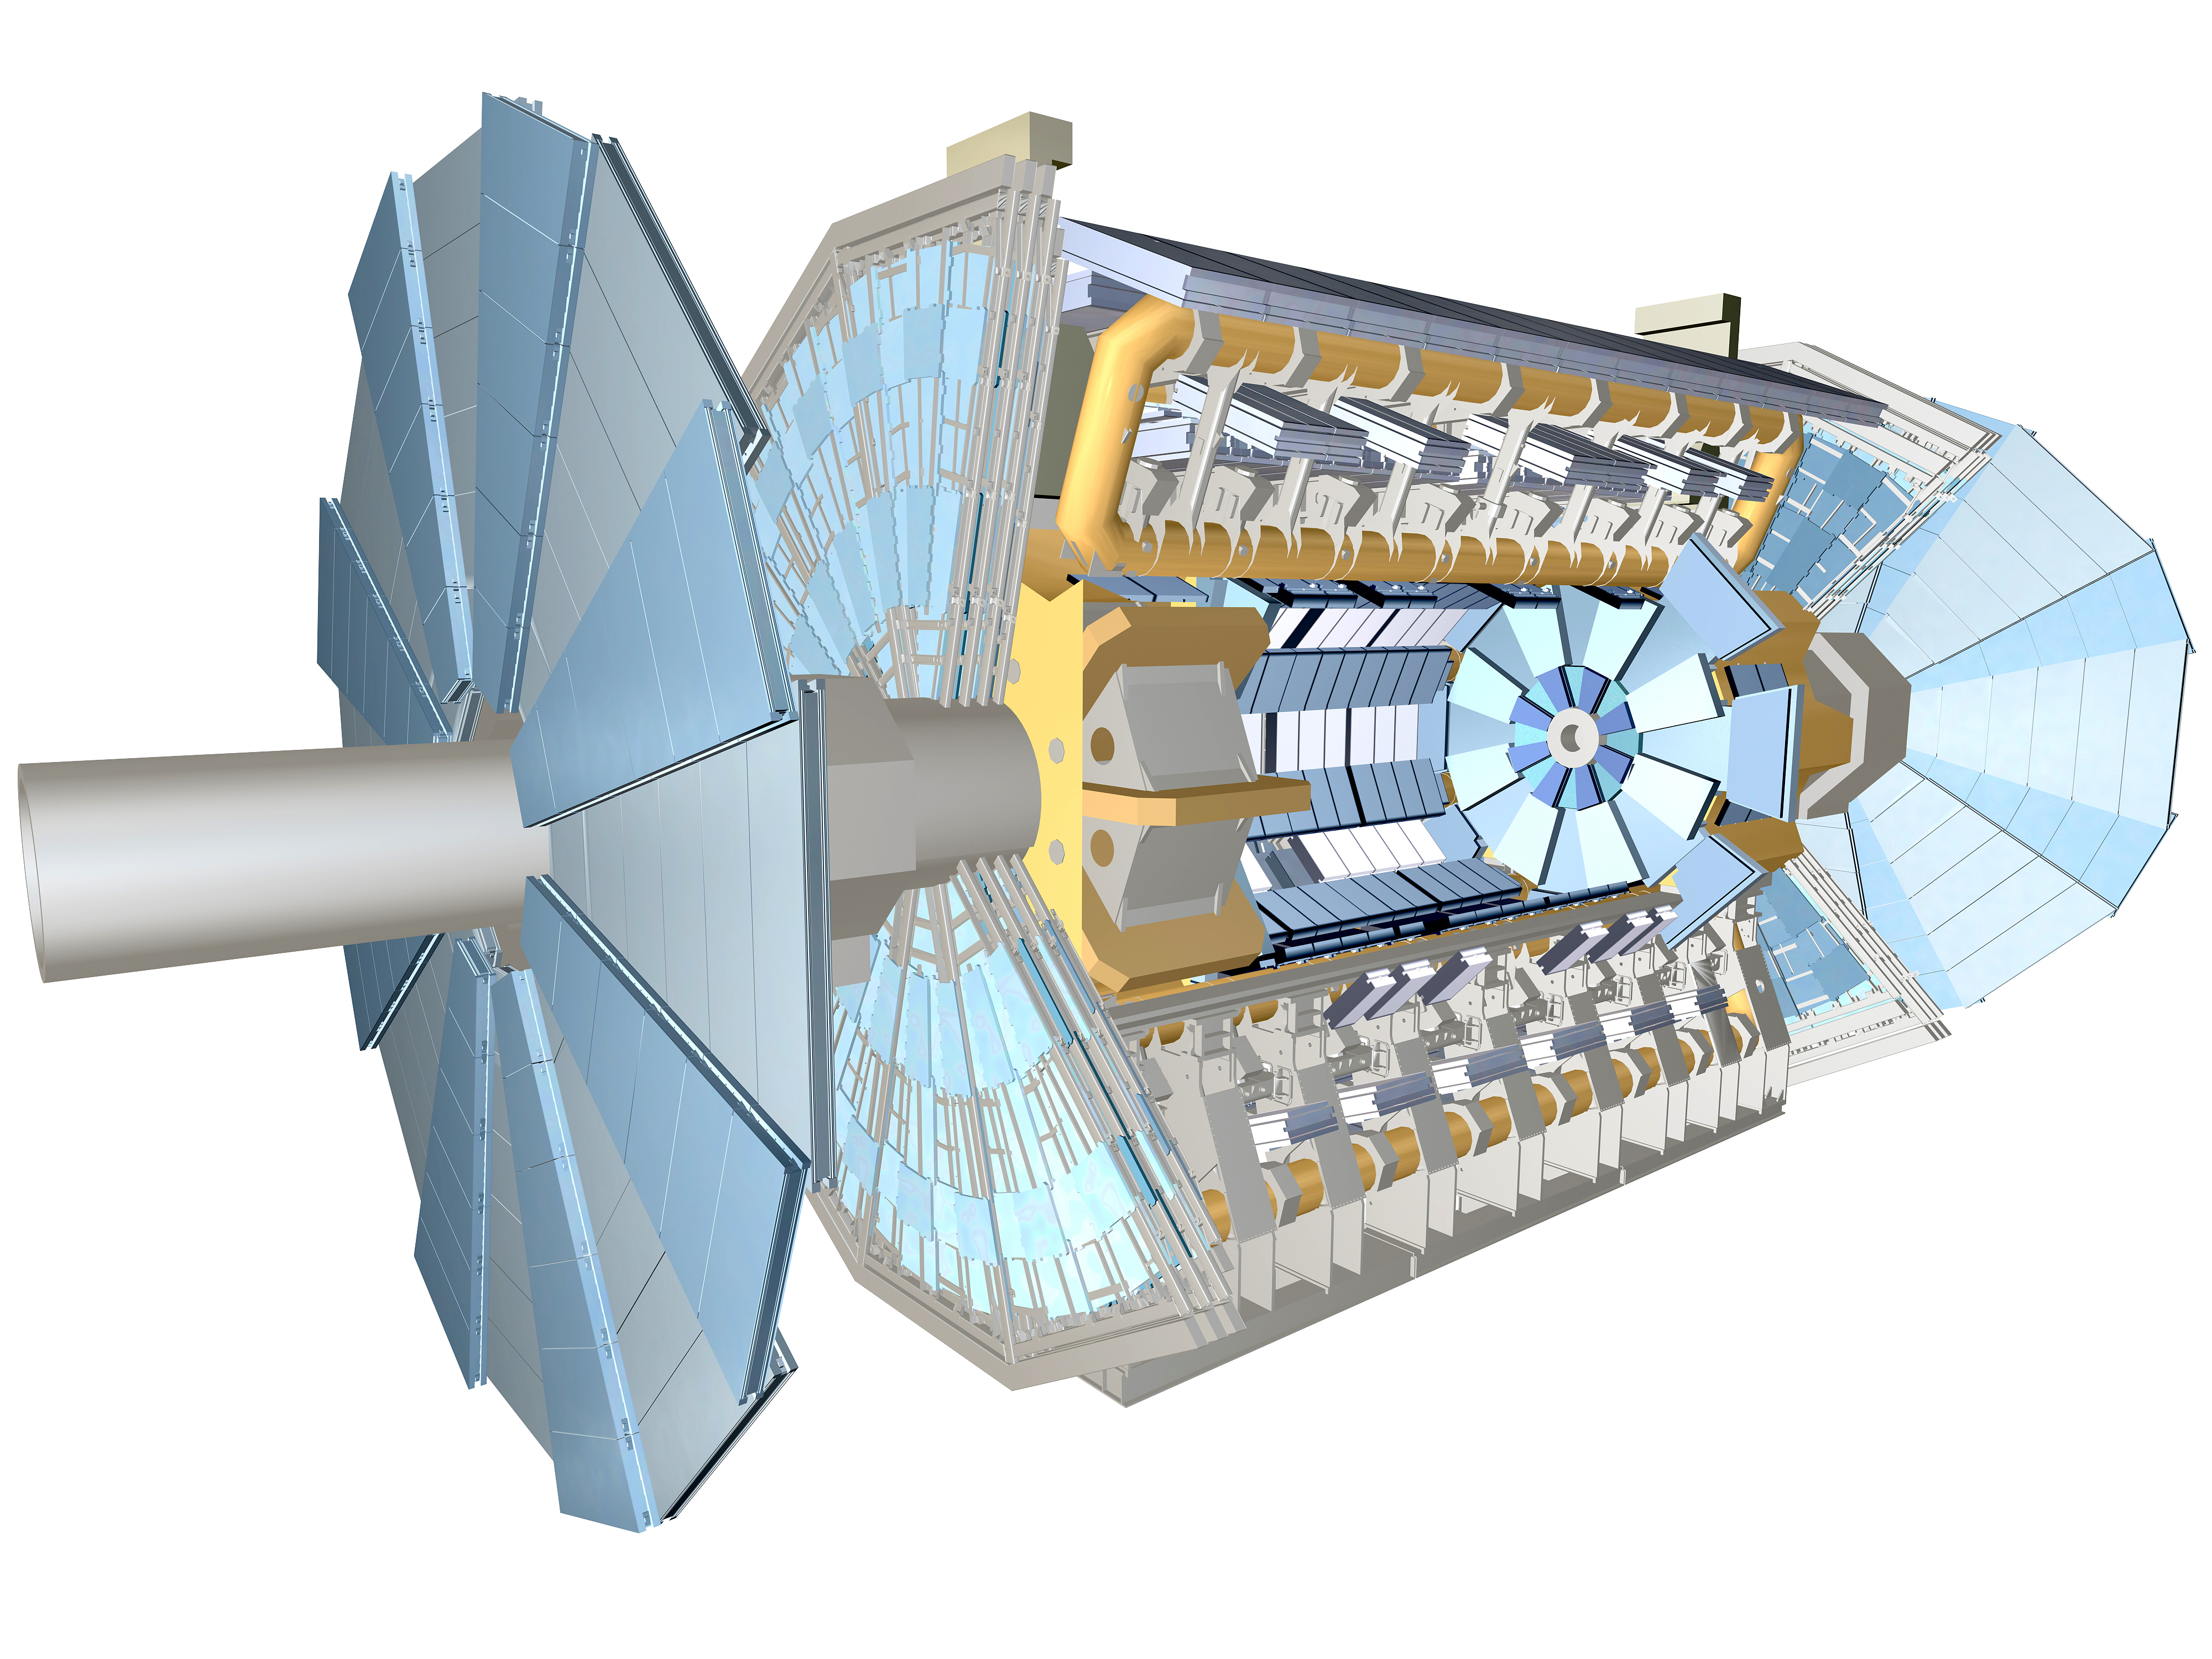
\includegraphics[width=\textwidth]{images/muons}};
        \node[anchor=east,align=center] (rpc) at ($(image.north east)+(-2.5,-0.5)$) {Resistive plate\\ chambers (RPC)};
        \draw (rpc.south) to (11,9.5);
        \draw (rpc.south) to (9.55,8.75);
        \draw (rpc.south) to (9.55,8.55);

        \node[anchor=west,align=center] (tgc) at ($(image.north west)+(5,0.5)$) {Thin gap\\ chambers (TGC)};
        \draw (tgc.south) to (6.95,8.4);
        \draw (tgc.south) to (7.1,8.5);
        \draw (tgc.south) to (7.35,8.8);

        \node[anchor=west,align=center] (mdt) at ($(image.south west)+(6,0.5)$) {Monitored drift\\ tubes (MDT)};
        \draw (mdt.north) to (5.2,3.2);
        % \draw[draw=red] (mdt.north) to ++(0.25,2);
        \draw (mdt.north) to (10,5.5);
        \draw (mdt.north) to (9.0,8.72);

        \node[anchor=east,align=center] (csc) at ($(image.south east)+(0,3)$) {Cathode strip\\ chambers (CSC)};
        \draw (csc) to ++(-2.75,3.65);
    \end{tikzpicture}
    \caption[Illustration of the ATLAS muon spectrometer components]{Illustration of the ATLAS muon spectrometer components.
    The toroid magnet coils are also shown in yellow~\cite{ATLASMuonImage}.}    
    \label{fig:method:ATLAS:muons}
\end{figure}

In the barrel toroid there are eight coils which provide bending the the region $\abs{\eta} < 1.4$ and in the region $1.6 < \abs{\eta} < 2.7$ the tracks are bent by two smaller end-cap magnets which are inserted into both ends of the barrel toroid. The transition region, $1.4 < \abs{\eta} < 1.6$ consists of a combination of barrel and end-cap fields which provide magnetic deflection. 

The muon spectrometer is composed of modules which use different detection technologies. These modules are organised into barrel and end-cap modules. Precise measurements of the $\eta$ position of the muons are performed in the barrel region by the \emph{monitored drift tubes} (MDTs) which allow for precise measurements of the muon momentum. The MDTs function similarly to the straw tube TRT in the ATLAS inner detector. They are formed of \SI{30}{\nano\meter} tubes with a central tungsten wire, which is filled with a gas mixture of Ar/CO$_2$ held at \SI{3}{\bar}. The MDT modules are located in and on the eight coils of the superconducting barrel toroid magnet. The first layer allows for a coverage $\abs{\eta} < 2.0$ and the second and third layers have a coverage of $\abs{\eta} < 2.7$. The MDT spatial resolution is \SI{80}{\micro\meter} and \SI{35}{\micro\meter} per chamber due to having multiple layers of tubes per chamber which provide multiple hits. 

The innermost layer consists of the \emph{cathod-strip chambers} (CSCs), located in the region $2.0 < \abs{\eta} < 2.7$. The CSC chambers are multi-wire proportional chambers with cathode planes segmented into strips in orthogonal directions in order to provide radial and transverse measurements. The space between the two planes is filled with a gas mixture mainly formed of Ar. Muons will ionise the gas, and positive ions are collected and read out by copper strips. The $\phi$ coordinate is measured by the time taken for the induced charges to drift to the cathode. CSC modules are formed of four stacked CSC planes, and these achieve a combined resolution of \SI{40}{\micro\meter} in the $\eta$ direction and \SI{4}{\milli\meter} in the $\phi$ direction.

Together the CSCs and the MDTs form the precision tracking chambers and provide state of the art precision measurements of the muon $p_{T}$. A muon $p_{T}$ resolution of $\sigma_{p_{T}}/p_{T} = 10 \% $ at  $p_{T} = \SI{1}{\tera\electronvolt}$ is achieved. 

Special chambers are used to trigger on muons. The fast muon chambers provide signals within \SI{25}{\nano\second} after the passage of a particle, which allows to tag the beam crossing. This measures both the coordinates of the track, in the bending plane ($\eta$) and the non-bending plane ($\phi$). In the barrel region, where $\abs{\eta} < 1.05$, \emph{resistive plate chambers} (RPC) are used which provide a resolution of \SI{10}{\milli\meter} in both the $z$ and $\phi$ directions. The RPCs are formed of two parallel plates made from a highly resistive plastic laminate with a gas mixture in between the plates. A strong electric field is placed between the resistive plates. The gas between the plates is ionised by passing muons, inducing an avalanche of electrons which creates a measurable signal in the form of current spikes in matrices of aluminium strips on the back of the resistive strips. In the end-cap region, where $1.05 < \abs{\eta} < 2.4$, \emph{thin gap chambers} (TGCs) are installed. Similar to the CSCs, the TCGs are multi-wire proportional chambers. For the TGC modules, the distance between the wire and strips is smaller than the distance between the wires, resulting in a smaller uniform region of the electric field. This allows for the electrons formed in the gas ionisation to drift to the wires faster. The TGCs provide muon track information with a precision of 2 - \SI{7}{\milli\meter} in the $\eta$ direction and 3 - \SI{7}{\milli\meter} in the $\phi$ direction.

\subsection{Trigger and Data Acquisition System}\label{sec:method:ATLAS:trigger}
The ATLAS trigger system is used to manage the high rate of LHC collisions, reducing the event rate from \SI{40}{\mega\hertz} to $\mathcal{O}$(\SI{100}{\kilo\hertz}) at which events can be written to mass storage. This is done by partially reconstructing events during data taking and identifying events of interest to record. The trigger system must balance a good rejection of background events while maintaining a high rate of interesting events being saved. A chain of decision-making algorithms in hardware and software is utilised. For Run-2, the ATLAS trigger system uses a two-level system; the Level 1 (L1) hardware trigger and the High-Level Trigger (HLT) software trigger. The data acquisition (DAQ) system controls the data flow when trigger decisions have been received. An overview of the components of the ATLAS trigger and DAQ systems outlined in \cref{fig:method:ATLAS:TDAQ}.
\begin{figure}[!htpb]
    \centering
    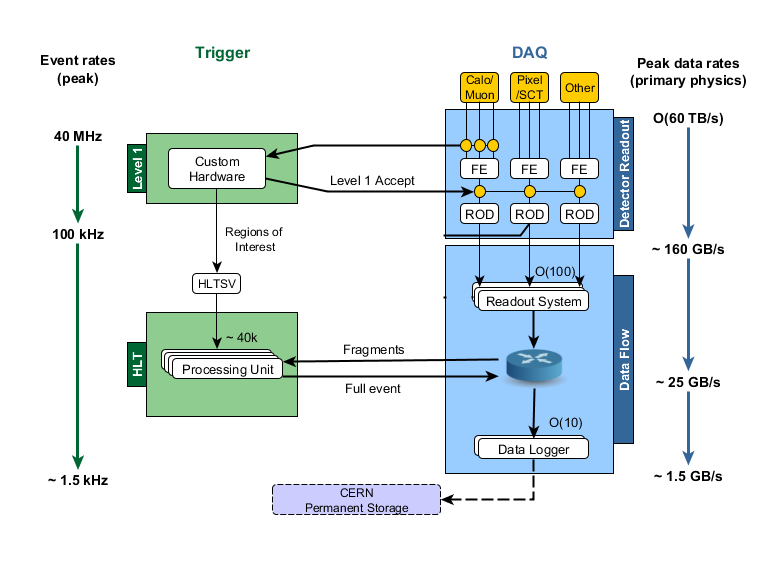
\includegraphics[width=\largefigwidth]{images/tdaqFullNew2017.png}
    \caption[Overview of the ATLAS trigger and data acquisition system]{Schematic overview of the ATLAS trigger and data acquisition system~\cite{ATLAS:TDAQ-Run2}.}
    \label{fig:method:ATLAS:TDAQ}
\end{figure}

\subsubsection{Level 1 trigger}
The hardware-based L1 trigger is designed to reduce the event rate from \SI{40}{\mega\hertz} to \SI{100}{\kilo\hertz}. Information from the muon trigger chambers and the calorimeters are used in the L1 trigger. The L1 trigger is divided into three parts: the L1 calorimeter trigger (L1Calo), the L1 muon trigger (L1Muon) and the central trigger processor (CTP).

The \emph{calorimeter trigger} relies on firmware-programmable FPGAs. On-detection electronics provide the sum of the analogue signals of hadronic and electromagnetic calorimeter cells in special trigger towers, with typical granularity of approximately $\Delta\eta \times \Delta\phi = 0.1 x 0.1$. The analogue signals are digitised by a preprocessor (PPr). Once the signals have been digitised, they are converted to $E_{T}$ using look-up tables, and a series of selections filter the event signatures for $e$, $\gamma$, hadronically-decaying $\tau$, and jets. The object counts that survive each threshold is passed to the CTP. 

The RPC and TGC of the muon spectrometer use a simple tracking algorithm to identify muon candidates who fall into six $p_{T}$ windows from \SI{5}{\giga\electronvolt} to \SI{35}{\giga\electronvolt}. The bunch crossing in which the signal originates can be determined from the time of flight due to the time resolution of the trigger chambers. The information from the RPC and TGC are combined in the muon-to CTP-interface (MuCTPI) and forwarded to the CTP. 

The \emph{topological trigger} system (L1Topo)~\cite{ATLAS:L1Topo} operates between L1Calo, L1Muon systems and the CTP. It receives input from the L1Calo and L1Muon systems in the form of trigger objects, combining the information and applying algorithmic cuts it can discriminate event topologies and shapes. The surviving trigger objects are passed to the CTP.

The CTP makes decisions on accepting or rejecting an event by combining the information from the trigger subsystems. It can be programmed with up to 96 trigger menu items that define different event selection rules. Additional requirements on prescale or deadtime can be used to reject events by the CPT further. Prescale requirements refer to trigger menu items that have been prescaled as to dampen the acceptance rate of events which pass the cuts. The time difference between L1 accept signals in which front-end drivers or HLT components of the trigger and DAQ system are saturated is referred to as deadtime. Regions of interest (RoIs) are identified by the L1 trigger which could contain high $p_T$ leptons, photons or jets and passed to the HLT, to reduce processing time. 

\subsubsection{High level trigger}
The ATLAS HLT~\cite{ATLAS:HLT-TDR,ATLAS:TDAQ-Run2} performs software-based reconstruction of events which pass the L1 trigger, running on processor farms consisting of 80000 CPU cores. The \emph{inner detector trigger} is responsible for the track reconstruction of measurements made by the inner detector. The reconstructed tracks are matched to measurements by the sub-detectors providing reconstruction of physics objects. This allows the HLT to differentiate between photons and electrons, and to tag jets which contain $b$ quarks. 

Due to the flexibility of software implementations and large-scale parallel processing, HLT algorithms can be more complicated than those in L1. HLT algorithms are combined into chains that are applied to the event data sequentially. These algorithms may use the RoIs provided by the L1 trigger, where the processing rate can be increased and reduce the latency. When an event survives an algorithm chain from the HLT, it is accepted and read out into permanent storage. An event rate of \SI{1}{\kilo\hertz} is achieved by the HLT.

\subsubsection{Trigger configurations}

The ATLAS trigger is based on many individual \emph{trigger chains}, referred to as triggers. The trigger system is configured to record collisions of interest, while limiting the processing load, allowing for a reasonable throughput. Each trigger defines selections on one or more reconstructed objects by the L1 trigger, followed by selection in the HLT trigger. Therefore, the HLT and L1 systems must use compatible modes of operations.

\section{Luminosity}\label{sec:method:lumi}

For a detector the total luminosity of collisions recorded, L, is given by, 
\begin{equation}
   \sigma L = N = \sigma \int_{}^{} \mathcal{L} dt,
\end{equation}

where N is the recoded number of events, $\sigma$ is the total inelastic cross section, and $\mathcal{L}$ is the instantaneous luminosity. $\mathcal{L}$ is given by~\cite{Herr}
\begin{equation}
    L = \frac{n_b f N_1 N_2 }{2\pi \Sigma_{x} \Sigma_{y}} F,
\end{equation}

where $f$ is the revolution frequency, $n_b$ is the number of colliding bunches with $N_{1(2)}$ protons, $\Sigma_{x(y)}$ the mean beam width in the x(y) direction. The luminosity detectors are calibrated to the inelastic cross section using van-der-Meer (VdM) scans ~\cite{ATLAS:Balagura_2011,ATLAS:vanderMeer:296752}.

The total luminosity delivered per data-taking period at $\sqrt{s} = $ \SI{13}{\tera\electronvolt} is shown in~\cref{fig:method:Lumi:lumirun2year}. The cumulative luminosity delivered by the LHC and recorded by ATLAS is presented in ~\cref{fig:method:Lumi:lumiRun2vsatlas}. Due to inefficiencies in data acquisition, the recorded luminosity is lower than what is delivered by the LHC.

\begin{figure}[]
    \centering
    \begin{subfigure}[b]{0.49\textwidth}
        \centering
        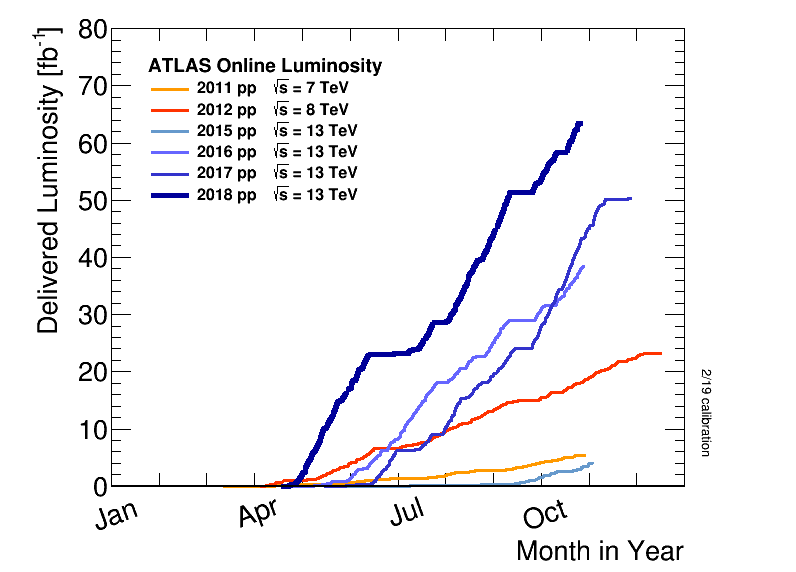
\includegraphics[width=\textwidth]{images/intlumivsyear.png}
        \caption{}
        \label{fig:method:Lumi:lumirun2year}
    \end{subfigure}
    \begin{subfigure}[b]{0.49\textwidth}
        \centering
        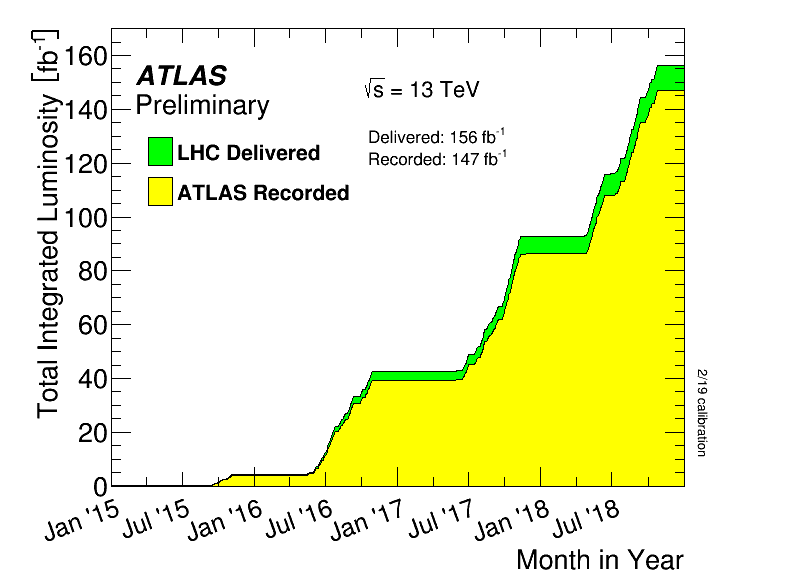
\includegraphics[width=\textwidth]{images/intlumivstimeRun2.png}
        \caption{}
        \label{fig:method:Lumi:lumiRun2vsatlas}
    \end{subfigure}
    \caption[Total Integrated Luminosity at Run-2 (13 TeV pp data only);
    Delivered Luminosity versus time for 2011-2018 (p-p data only)]{(a) Cumulative luminosity versus time delivered to ATLAS (green) and recorded by ATLAS (yellow) during stable beams for pp collisions at 13 TeV centre-of-mass energy in LHC Run-2. (b) Cumulative luminosity versus day delivered to ATLAS during stable beams and for high energy p-p collisions~\cite{ATLAS:lumiPlots}.}
    \label{}
\end{figure}

\clearpage